%\section{Attack on \present}
%	In \cite{DBLP:conf/asiacrypt/XiangZBL16} authors found a five round distinguisher on \present. They have shown that if they fix the left most 60 bits as random constant and varry the right most 4 bits then after 5 rounds the right most 4 bits are coming as balanced. But they didnot mention one interesting thing about this property, that after 5 rounds the same 4 bits will be balanced even if we varry the 4 bits input. Without giving All property at the right most 4 bits if we give the All property at input of any \sbb then also the same right most 4 bits will be balanced. The same thing we can observe on the smaller versions of \present. The balanced bits of different versions of \present have shown in table \ref{tab:present_versions_balanced_bits}. At \present-32, after 4 rounds the bits ... are balanced. At \present-16 after 4 rounds 0-th bit is balanced. We can verify this using monomial representation. For \present-16, in the monomial representation of the 0-th bit after 4 rounds we can see that the monomials $x_0x_1x_2x_3, ~x_4x_5x_6x_7, \cdots, ~x_{12}x_{13}x_{14}x_{15}$ are not present. For this reason if we give the All property at the inputs of an \sbb then after 4 rounds 0-th bit becomes balance.
%	
%	\begin{center}
%		\begin{table}[h]
%			\begin{Tabular}[1.3]{|c|c|c|c|}
%				\hline
%				\present version & msg size & round & balanced bits	\\
%				\hline
%				16 & $2^4$ & 5 & 0,1,2,3 \\
%				8 & $2^4$ & 4 &  \\
%				4 & $2^4$ & 4 & 0 \\
%				\hline
%			\end{Tabular}
%			\caption{balanced bits at different versions of \present}
%			\label{tab:present_versions_balanced_bits}		
%		\end{table}
%	\end{center}
%	
%	\paragraph{Interchanging ANF of \present.}
%	Original ANF of \present is 
%	$$\begin{cases}
%		& y_0 = x_0 \oplus x_2 \oplus x_3 \oplus x_1x_2	\\
%		& y_1 = x_1 \oplus x_3 \oplus x_1x_3 \oplus x_2x_3 \oplus x_0x_1x_2 \oplus x_0x_1x_3 \oplus x_0x_2x_3	\\
%		& y_2 = 1 \oplus x_2 \oplus x_3 \oplus x_0x_1 \oplus x_0x_3 \oplus x_1x_3 \oplus x_0x_1x_3 \oplus x_0x_2x_3	\\
%		& y_3 = 1 \oplus x_0 \oplus x_1 \oplus x_3 \oplus x_1x_2 \oplus x_0x_1x_2 \oplus x_0x_1x_3 \oplus x_0x_2x_3	\\
%	\end{cases}$$
%	
%	If we interchange the positions of $y_0, y_1, y_2, y_3$ then from mini \present we can see the position of the balanced bit is shifting after four rounds. In particular it depends upon the bit that we placed at the position of $y_0$. In table \ref{tab:anf_permutation} we have given the positions of the balanced bits that depends upon the permutation of $y_0, y_1, y_2, y_3$. 
%	
%	\begin{center}
%		\begin{table}[!h]
%			\begin{Tabular}[1.3]{|c|c|}
%				\hline
%				\texttt{ANF} at $y_0$ & balanced bit position	\\
%				\hline
%				$y_0$ & 0 \\
%				$y_1$ & 5 \\
%				$y_2$ & 10 \\
%				$y_3$ & 15 \\
%				\hline
%			\end{Tabular}
%			\caption{balanced bit position after ANF permutation of \present}
%			\label{tab:anf_permutation}		
%		\end{table}
%	\end{center}
%	
%	
%\section{Balanced Bits of \present-64 and \gift-64.}
%The Balanced bits of \present and \gift are given in table \ref{tab:present_balaned_bits} and \ref{tab:gift_balaned_bits} resp. For 5 rounds of \present if we active input 4 bits of any \sbb then at output the bits number 0,1,2,3 will be balanced. Similarly the balanced bits after 3 rounds of \present with 2 active bits are given in tab \ref{tab:present_balaned_bits}. For 5 rounds of \gift, if we active 4 bits of any \sbb input then we will get the corresponding balanced bits given in tab \ref{tab:gift_balaned_bits}. Another one interesting property within tab \ref{tab:gift_balaned_bits} is the 3 rounds with 1 active bit. If we consider 1 active bit at bit numbers 28, 29, 30, 60, 61, 62 then depending upon the position of the active bits total 16 bits will be balanced. We get 2 sets of balanced bits. One for bit numbers 28, 60 and other for bit numbers 29, 30, 61, 62. This can be visualize as a generalization of differential property also. In terms of fault attack this can be very useful. For fault in 1 active bit we just have to give 1 fault at that particular bit position. 
%	\begin{center}
%	\begin{table}[!h]
%		\begin{Tabular}[1.3]{|c|c|c|c|}
%			\hline
%			round & \# active bits & \#balanced bits & balanced bits position	\\
%			\hline
%			5 & 4 & 4 & 0,1,2,3	\\
%			5 & 3 & 0 &		\\
%			\hline
%			4 & 4 & 64 & 0(1)64	\\
%			4 & $3^\ast$ & 16 & 0(1)16	\\
%			\hline
%			3 & $2^\ast$ & 16 & 0, 4, 8, 12, 16, 20, 24, 28, 32, 36, 40, 44, 48, 52, 56, 60	\\
%			3 & $2^\ast$ &16 &2, 6, 10, 14, 18, 22, 26, 30, 34, 38, 42, 46, 50, 54, 58, 62	\\
%			3 & 1 & 0 &	\\ 
%			\hline
%		\end{Tabular}
%		\caption{balanced bit position after last p-layer of \present-64}
%		\label{tab:present_balaned_bits}		
%	\end{table}
%\end{center}
%
%
%
%\begin{center}
%	\begin{table}[!h]
%		\begin{Tabular}[1.3]{|c|c|c|c|}
%			\hline
%			round & \# active bits & \#balanced bits & balanced bits position	\\
%			\hline
%			5 & 4 & 16 & 0, 4, 8, 12, 16, 20, 24, 28, 32, 36, 40, 44, 48, 52, 56, 60$\ast$	\\
%			5 & 3 & 0 &		\\
%			\hline
%			4 & 4 & 64 & 0(1)64	\\
%			4 & $3^\ast$ & 24 & $\ast$	\\
%			\hline
%			3 & $2^\ast$ &  & $\ast$	\\
%			3 & $1\ast$ &16 & 3, 7, 11, 15, 16, 20, 24, 28, 33, 37, 41, 45, 50, 54, 58, 62	\\
%			3 & $1^\ast$ &16 & 0, 4, 8, 12, 17, 21, 25, 29, 34, 38, 42, 46, 51, 55, 59, 63	\\
%			\hline
%		\end{Tabular}
%		\caption{balanced bit position after last p-layer of \gift--64}
%		\label{tab:gift_balaned_bits}		
%	\end{table}
%\end{center}
%
%%
%%(i) Div prop in terms fault
%%(ii) same balanced bits in smaller versions of present and gift
%%(iii) attack algorithms
%%(iv) toy cipher monomial view, the 
%%(v) 2 round decryption of GIFT
%
%
%\section{Monomial prediction}

%
%
%\section{MILP based model of present and gift to prove the balanced bits at the same positions}
%
%
%In \cite{DBLP:conf/asiacrypt/XiangZBL16} authors used Mixed Integer Linear Programming (MILP) to model the Division property of \present-64. They have shown the Division Trails (DT) of the cipher and use sagemath to make equations that satisfy the trails. For \present-64 the linear layer is only bit permutation. Authors used the inequalities that represents DT and bit permutations to model it. They set some bits to 1 initially that represents of giving All property at those bit positions. After some rounds they checked the bits that are becomes balanced.
%
%In this work for the ciphers \present and \gift we have given the All property to the input bits of each nibble individually and get the balanced position after 5 rounds. If we varry the nibble position i.e. giving the All property at any random nibble, then also the balanced bits occurs at the same position after 5 rounds. The fixed balanced bits position of the ciphers are given in the table \ref{tab:present_balaned_bits} \ref{tab:gift_balaned_bits}. This behaviour is coming as in the monomial expression after 5 rounds of \present the product of input four bits of any nibble is not present. For \present-64 it is difficult to generate the algebraic expression of the whole cipher after 5 rounds. However there are some smaller versions of \present which have shown in the paper \cite{DBLP:journals/iacr/Leander10}. The algebraic expression of \present version 4 can be generated in sagemath. In there we have found if we varry the nibble randomly where the All property has been given, the bit 0 after 4 rounds remains balanced. We have generated the algebraic expression of bit 0 after 4 rounds and verify that the input bits of any \sbb (i.e. $x_{4i}~x_{4i+1}~x_{4i+2}~x_{4i+3}$, for $i$ in range\{16\}) is not present in the expression. This is shown in section \ref{present_small_versions_balanced_bit}. 


\section{Balancedness in \present cipher}	\label{sec:present_random_nibble_explanation}
In this section, we look into a new property of the cipher \present. This is a 5 rounds random nibble property of the block cipher. Here we give All property at any random nibble in the input. As a result, we get balanced bits at fixed positions after 5 rounds. We illustrate the active bit propagation and the monomial view of the propagated bits by \autoref{fig:present_active_bit_propagation}. Suppose we give the All property at the input of the 0th nibble. Therefore whenever in the ANF (Algebraic Normal Form) representation of a bit, the product term $x_3x_2x_1x_0$ comes, that bit will be balanced. After the \sbb of the 1st round, the anf representation of the bits becomes $y_3y_2y_1y_0$, where \begin{align*}
	& y_0 = x_0 \oplus x_2 \oplus x_3 \oplus x_1x_2	\\
	& y_1 = x_1 \oplus x_3 \oplus x_1x_3 \oplus x_2x_3 \oplus x_0x_1x_2 \oplus x_0x_1x_3 \oplus x_0x_2x_3	\\
	& y_2 = 1 \oplus x_2 \oplus x_3 \oplus x_0x_1 \oplus x_0x_3 \oplus x_1x_3 \oplus x_0x_1x_3 \oplus x_0x_2x_3	\\
	& y_3 = 1 \oplus x_0 \oplus x_1 \oplus x_3 \oplus x_1x_2 \oplus x_0x_1x_2 \oplus x_0x_1x_3 \oplus x_0x_2x_3	\\
\end{align*}

After the permutation, the active bits go to the 0th bit of the nibbles 0,4,8,12 respectively. The other bits of that round are inactive. Hence at the output of the 2nd round, only the output bits of the nibble number 0,4,8,12 are active. At 3rd round, the ANF representation of the bits of 0th bit of each \sbb is $c_i + c_j y_k$, where $c_i, c_j's$ are constant and $k$ varies in range(3).


\begin{figure}[!h]
	\centering
	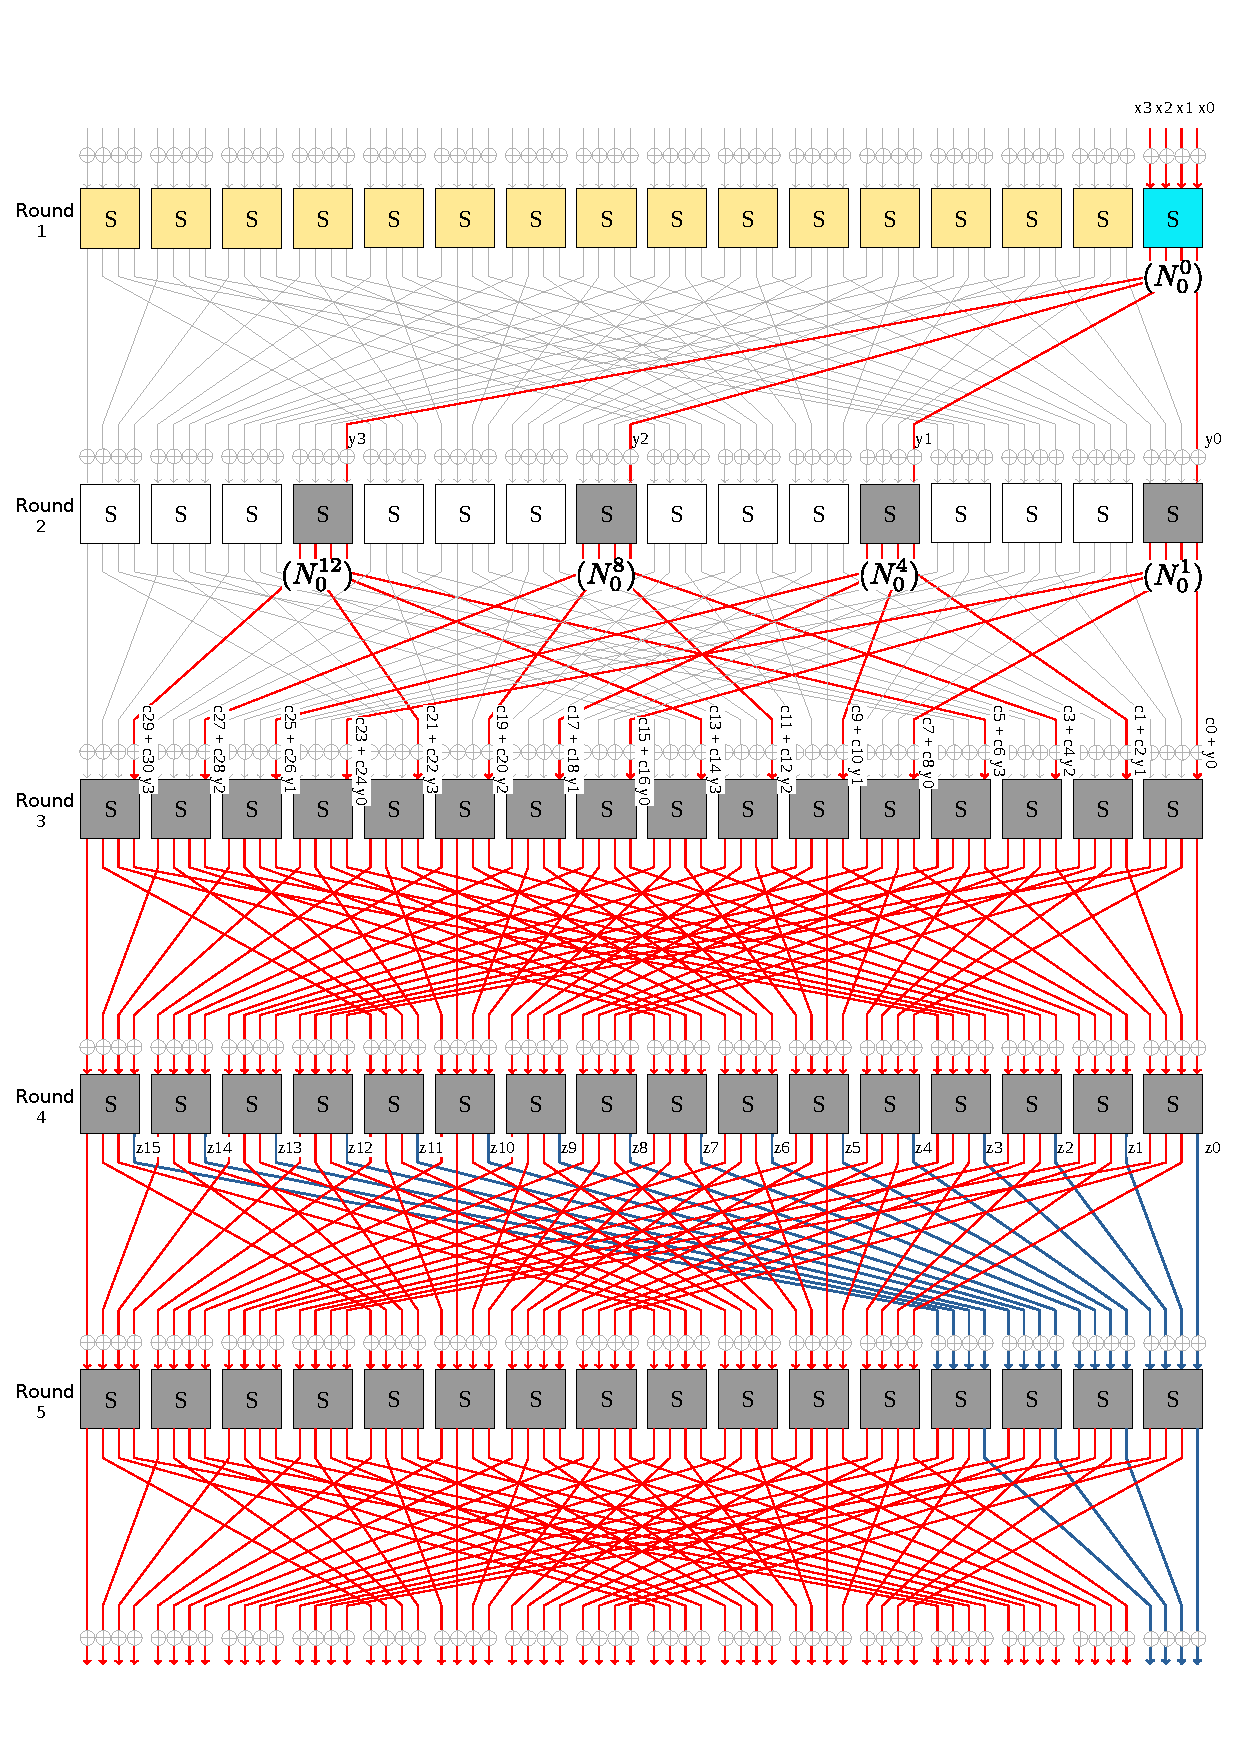
\includegraphics[width=\linewidth]{fig/present_cipher_active_bit_propagation.pdf}
	\caption{active bit propagation on \present}
	\label{fig:present_active_bit_propagation}
\end{figure}


Hence at the output of the 2nd round, only 16 bits are active. Up to this point, the active bit's ANF representation does not contain the product term $x_3x_2x_1x_0$, so the constant bits as well as the active bits are balanced. Interestingly the 16 active bits go into the 0th input bit of 16 \sbb s in the 3rd round. At the output of the 3rd round, all 64 bits become active. In the input of the 4th round, each \sbb contains one bit dependent upon $y_3, y_2, y_1, y_0$ respectively. Therefore at the output of the 4th round, there will be $z_i's$; where each $z_i$ is a combination of $y_3y_2y_1y_0$. Though at this point, the ANF of each $z_i's$ contains $y_3y_2y_1y_0$ i.e. a combination of $x_3x_2x_1x_0$ but the product term $x_3x_2x_1x_0$ is not there. At the output of round 4, we see only the 0th bit of each \sbb. This is because only the ANF representation of the 0th bit contains a maximum 2-degree term. Whereas the other bits are of the 3-degree term. Therefore for other bits, their chance of producing the product term $x_3x_2x_1x_0$ is higher. The 0th bit of each \sbb after the 4th round goes to the input of the initial 4 \sbb s in the input of the 5th round. Again we see in the next round (i.e. 5th round), that for the 0th bit of \sbb number 0,1,2,3 the chance of containing the term $x_3x_2x_1x_0$ is less than the other bits as in the previous round also they are coming from the 0th bits and in this round also they are the 0th bit of \sbb 0,1,2,3. We implemented this in Sagemath and verify that the anf representation of 0,1,2,3 bits only (after 5 rounds permutation) does not contain the product term $x_3x_2x_1x_0$. The other bit's ANF representation contains it. Therefore after 5 rounds, the bits 0,1,2,3 becomes balanced. 



\begin{figure}[!h]
	\centering
	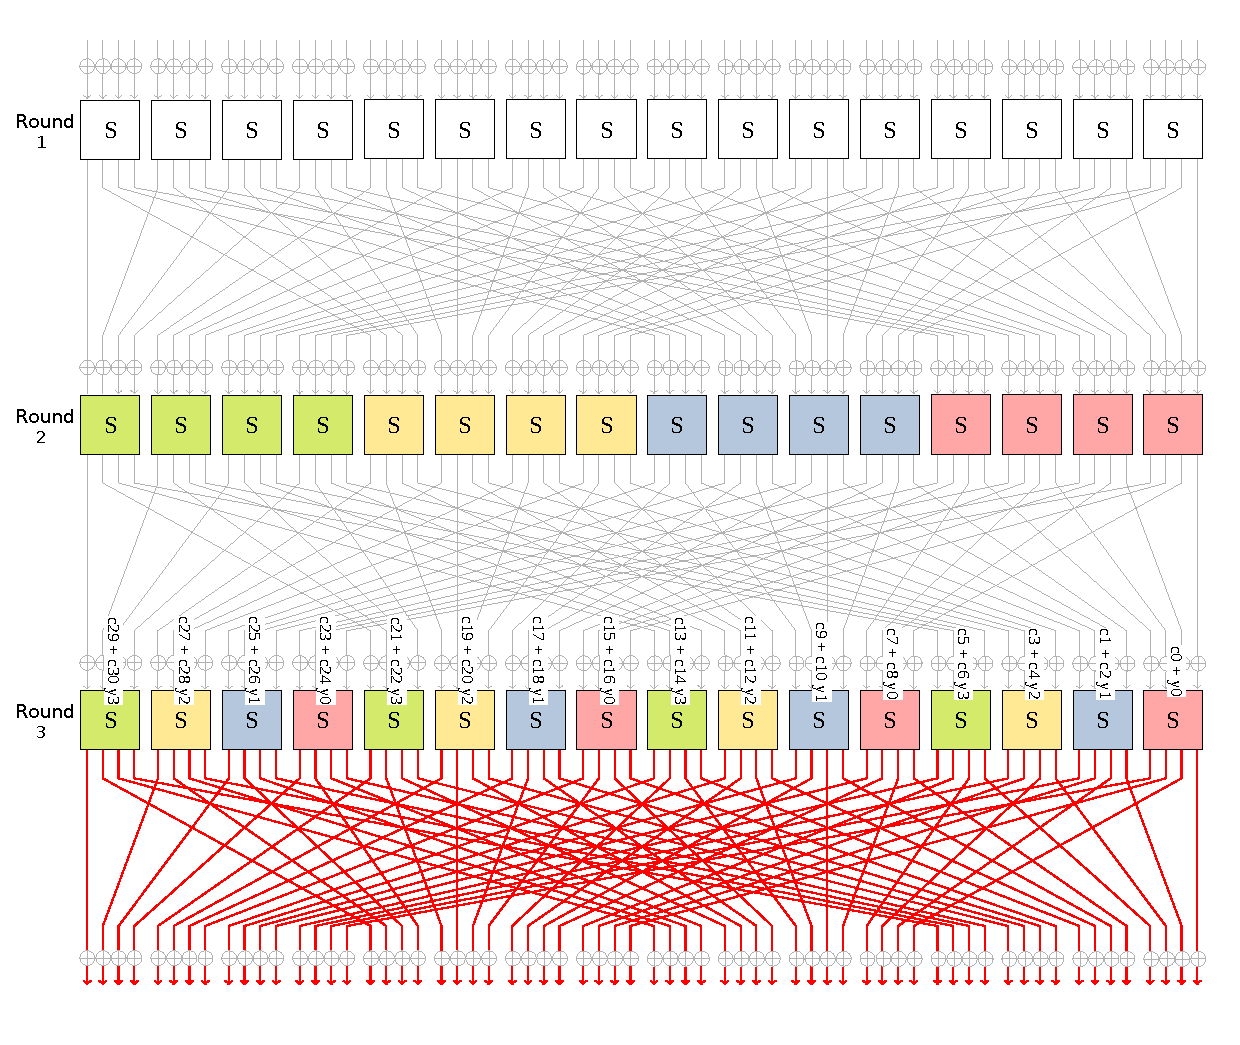
\includegraphics[width=\linewidth]{fig/present_cipher_active_bit_propagation_random_nibble.pdf}
	\caption{random nibble active bit propagation on \present}
	\label{fig:present_active_bit_propagation_random_nibble}
\end{figure}


We have shown the 4 bits become balanced after 5 rounds if we give the All property at the input of the 0th nibble. Now we show if we give the All property at the input of any \sbb then also after 5 rounds the same 4 bits remain balanced. For this claim, we show that if we give All at any \sbb then also at the output of the 3rd round the ANF representation of the bits are the same, just the constants vary. We illustrate this from \autoref{fig:present_active_bit_propagation_random_nibble} . In \autoref{fig:present_active_bit_propagation_random_nibble}, we can see that irrespective of the nibble position of All property, due to present permutation 0th bit always goes to one of the red nibbles in round 1. Similarly, 1st bit, 2nd bit, and 3rd bit of the All property go to one of the blue, yellow, and green ones in the 2nd round. Hence because of the present permutation layer one of each colored \sbb in \autoref{fig:present_active_bit_propagation_random_nibble} becomes active in the 2nd round, where red, blue, yellow and green one contains constant combination of $y_0$, $y_1$, $y_2$, $y_3$ respectively. From each red \sbb, one bit goes to red ones in the 3rd round. The same thing happens for other colors also in round 2. Therefore in the input of 3rd round constant combination of $y_0, y_1, y_2, y_3$ goes to nibble $4i, 4i+1, 4i+2, 4i+3$ for $i$ in range(3) respectively. Hence in the output of the 3rd round, the anf representation of bits will be similar (without constants) irrespective of where the All property has been given. So, after 5 rounds we always get the balanced bits at the same position despite of varying the All property position.
 


%
%
%\begin{algorithm*}[htbp]
%	\caption{\textsc{Key Recovery} ($C^\prime_1, \cdots, C^\prime_{16}$)}
%	\label{alg:key_recovery}
%	\begin{algorithmic}[1]	
%		\State Initialize a 2-dimensional array called key\_ctr	
%		\For{each key\_nibble in range\{$4$\}}	\Comment{key val of each nibble can be in \{0, 1, 2, 3\}}
%			\For {each $j$ in range \{$0$ - $16$\}}
%				\State dec\_msg[j] $\gets$ $SB^{-1}$(key\_nibble$\oplus$ $\text{perm}^{-1}(C^\prime_j$))	\Comment{can be done independently for nibbles}
%			\EndFor
%			xor\_sum $\gets$ dec\_msg[0] $\oplus$ $\cdots$ $\oplus$ dec\_msg[15]
%			\If{(xor\_sum \& \texttt{0x1}) is 0}	\Comment{checking last bit of xor\_sum is zero or not}
%				\State key\_ctr[nibble] $\gets$ key\_ctr[nibble] $\cup$ \{key\_nibble\} 
%			\EndIf
%		\EndFor
%		\State make all possible keys from key\_ctr
%		\For{each \sbb in the second last layer}			
%			\For{each possible\_last\_round\_key from key\_set}
%				\State choose \sbbes from last layer that comes from same $i$-th \sbb from the second last layer
%				\For{each key\_nibble in range \{4\}}	\Comment{for 2nd last layer}
%					\For{$j$ in range \{16\}}
%						\State dec\_msg[$j$] $\gets$ decrypt $C^\prime_j$ for two rounds using possible\_last\_round\_key and key\_nibble
%						\EndFor
%					xor\_sum $\gets$ dec\_msg[0] $\oplus$ $\cdots$ $\oplus$ dec\_msg[15]
%					\If{$i$-th nibble of xor\_sum is not 0}
%						\State miss\_count++	\Comment{If for each key\_nibble XOR is not 0 at $i$-th position before two rounds then key\_nibble choice is false}
%					\EndIf
%					\If{miss\_count is 4}
%						\State remove possible\_last\_round\_key from key\_list
%					\EndIf
%				\EndFor	
%			\EndFor	
%		\EndFor	
%	\Return key\_list			
%	\end{algorithmic}
%\end{algorithm*}
%
%\newpage


\section{\present key recovery attack}
In this section, we describe our last round key recovery attack on \present 64 using 5 round random nibble fault model.

\subsection{1 round key recovery attack}

\subsubsection{Distinguisher model}
To recover the last round key, we will use our 5 round random nibble fault model, which is described in \autoref{sec:present_random_nibble_explanation}. Our model is random nibble fault i.e. if we give All property at any random nibble then also the same 4 bits of 0th nibble will be balanced after 5 rounds. For this attack, we give 16 faults on a random nibble at input of 25th round. As our attack will work on any random nibble, so for the convention we assume we are giving fault to generate 16 faulty ciphertexts at 0th nibble we describe our key recovery attack in the next section.


\subsubsection{Key Recovery attack}
As described in the previous section, we are giving 16 faults to generate the All property at the 0th nibble in the input of the 25th round. We will get 4 balanced bits at the end of the 30th round. Using 16 faulty ciphertexts we recover 4 key bits of the last round. For this we choose those 4 bits which are coming from 0th nibble at 31-st round ($N_0^{31}$ in \autoref{fig:key_recovery_1_round_present}). We choose all possible 16 values of these 4 key bits. For each possible key value, we decrypt for one round of the ciphertexts. Then check for which key values, after inverting 1 round of 15 faulty ciphertexts and 1 ciphertext, the input 4 bits of $N_0^{31}$ is 0. We will take those keys as possible keys of the last round selected 4 bits of fig. \ref{fig:key_recovery_1_round_present}.

\subsubsection{Complexity}

In this 1 round attack of \present, we recover 4 bits of the last round uniquely. Here for each key nibble, we have to decrypt 16 faulty ciphertexts. Therefore time complexity of this attack = $2^8$. For this, we have to store 16 faulty ciphertexts. So the data complexity of this attack will be $2^4$. In algorithm \ref{alg:key_recovery_1_round_present} we are storing the possible nibble values of the key to a key list. But instead of storing those nibble keys, we can print those values. Then we do not have to store any value. So, the memory complexity of the attack is negligible.


\begin{figure}[!h]
	\centering
	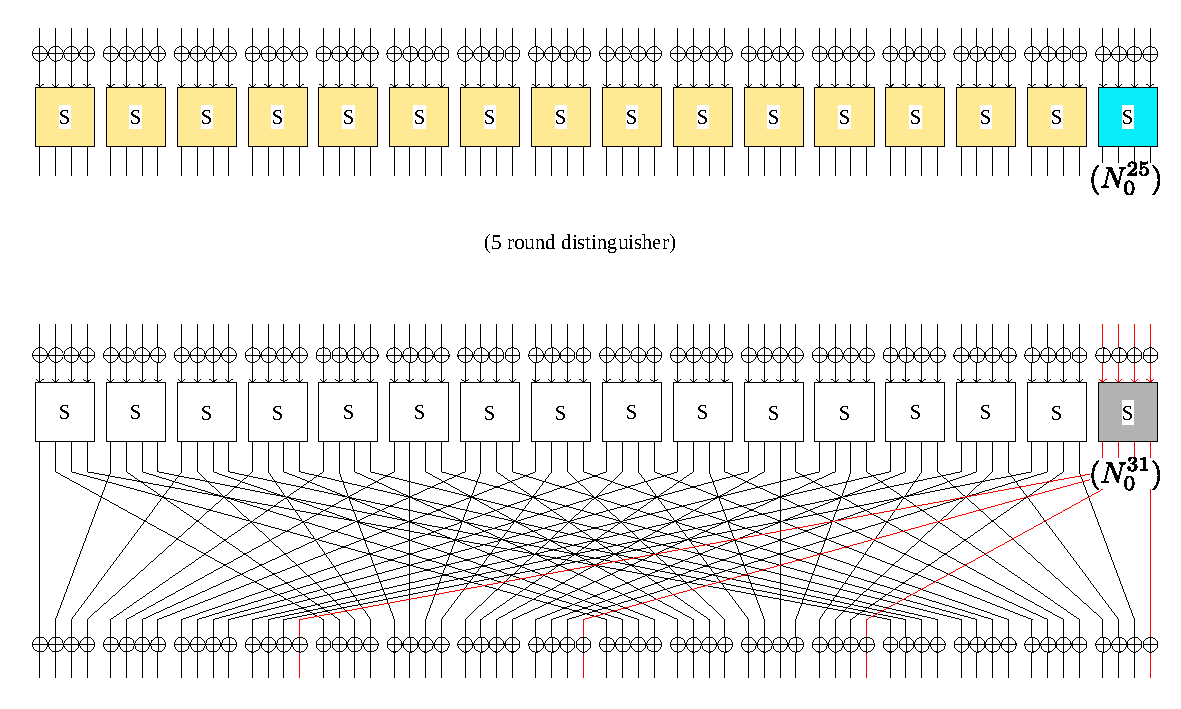
\includegraphics[width=\linewidth]{fig/spn_code_libra_1_round_attack.pdf}
	\caption{1 round key recovery attack on \present}
	\label{fig:key_recovery_1_round_present}
\end{figure}




\begin{algorithm*}[htbp]
	\caption{\textsc{Key Recovery} ($C^\prime_1, \cdots, C^\prime_{16}$)}
	\label{alg:key_recovery_1_round_present}
	\begin{algorithmic}[1]	
		\State Initialize an array called key\_list	
		\For{each key\_nibble in range\{$0$ - $16$\}}	\Comment{output of $SB$ at $N_0^6$ in fig.  \ref{fig:present_key_recovery_1_round}}
		\For {each $j$ in range \{$0$ - $16$\}}
		\State dec\_msg[j] $\gets$ $SB^{-1}$(key\_nibble$\oplus$ $\text{perm}^{-1}(C^\prime_j$))
		\EndFor
		xor\_sum $\gets$ dec\_msg[0] $\oplus$ $\cdots$ $\oplus$ dec\_msg[15]
		\If{first 4 bits of xor\_sum is 0}	\Comment{input of $SB$ at $N_0^6$ in fig. \ref{fig:present_key_recovery_1_round}}
		\State store \{key\_nibble\} in key\_list
		\EndIf
		\EndFor
		\Return key\_list			
	\end{algorithmic}
\end{algorithm*}




\subsection{2 rounds key recovery attack}
In this section, we discuss the 2 round attack on \present 64. We use our 5-round random nibble fault model distinguisher to recover some bit information of the last and 2nd last round key.

\subsubsection{Distinguisher model}
We use the same distinguisher model as discussed in the section \ref{sec:present_random_nibble_explanation}. Here we give 15 faults to generate 15 faulty ciphertexts and alongside generate the original ciphertext of the message. So we have in total 16 ciphertexts. In this case, we give All property in a nibble at the input of the 24th round as shown in \autoref{fig:key_recovery_2_round_present}. As our attack works on any random nibble so here also for the convention we give the All at 0th nibble of input of 24th round i.e. input of $N_0^{24}$. We discuss our key recovery attack in the next part of this section.


\subsubsection{Key Recovery attack}
Here we give fault to generate 16 ciphertexts at input $N_0^{24}$ in \autoref{fig:key_recovery_2_round_present}. By our attack model, we get the 4 initial bits as balanced after 5 rounds. So we get the balanced bits at input of 0th nibble in the 30th round i.e. $N_0^{30}$ in \autoref{fig:key_recovery_2_round_present}. We guess the 16 key bits of the last round and 4 key bits of the 2nd last round. We maintain a counter, ctr to keep track of the possible key values. Initially, we put the ctr value to 1 i.e. we consider all the 20-bit key values [16 for the last round and 4 for the 2nd last] as possible keys. If the possible keys do not satisfy our condition then we put the ctr value of the corresponding key as 0. Now for the last 4 nibble of keys i.e. output of the \sbb of $N_{31}^{12}, N_{31}^{8},N_{31}^{4},N_{31}^{0}$ in \autoref{fig:key_recovery_2_round_present} we guess all possible $2^{16}$ values of them and decrypt one round. Then we use 4 key bits of 30th round's 0th nibble i.e. output of $N_{0}^{30}$ in \autoref{fig:key_recovery_2_round_present} and decrypt the 16 ciphertexts for one more round. We check whether at the input of $N_{0}^{30}$ in \autoref{fig:key_recovery_2_round_present} the xor value of 16 decrypt ciphertexts becomes 0 or not. If it does not become 0 then we update the corresponding ctr value to 0. At last, we take those values of keys as possible keys for which the ctr value remains 1.
 
\begin{algorithm*}[htbp]
	\caption{\textsc{Key Recovery} ($C^\prime_1, \cdots, C^\prime_{16}$)}
	\label{alg:key_recovery_2_rounds_present}
	\begin{algorithmic}[1]	
		\State Initialize an array called key\_ctr of size $2^{20}$
		\State extract 16 bit last round keys and 4 bit 2nd last round keys
		\For{each key\_nibble in last\_round\_key}	\Comment{output of $SB$ at $N_0^{31}, N_4^{31}, N_8^{31}, N_{12}^{31}$ in \autoref{fig:key_recovery_2_round_present}}
		\For {each $j$ in range \{$0$ - $16$\}}
		\State dec\_msg[j] $\gets$ $SB^{-1}$(key\_nibble\_last\_round$\oplus$ $\text{perm}^{-1}(C^\prime_j$))
		\EndFor
		\For{each key\_nibble in 2nd\_last\_round\_key}	\Comment{2nd round decryption}
		\For {each $j$ in range \{$0$ - $16$\}}
		\State dec\_msg[j] $\gets$ $^{-1}$(key\_nibble\_2nd\_last\_round$\oplus$ $\text{perm}^{-1}(\text{dec\_msg[j]})$)	
		\EndFor
		\EndFor		
		xor\_sum $\gets$ dec\_msg[0] $\oplus$ $\cdots$ $\oplus$ dec\_msg[15]
		\If{first 4 bits of xor\_sum is 0}	\Comment{input of $SB$ at $N_0^{30}$ in \autoref{fig:key_recovery_2_round_present}}
		\State store \{key\_nibble\} in key\_list
		\EndIf
		\EndFor
		\Return key\_list			
	\end{algorithmic}
\end{algorithm*} 
 

\subsubsection{Complexity}
In our two rounds key recovery attack for \present, we use all possible keys of the nibble 0, 4, 8 and 12 to decrypt one round in the last layer. This can be done in parallel. As we have 16 messages, we need $2^{4+4} = 2^8$ computations to invert the last layer. In the 2nd layer, we have to do again $2^4$ many messages which are $2^8$. The xor sum and checking of 1ast 4 bits takes a constant amount of time. Therefore total time complexity = $\mathcal{O}(2^8)$. This reduces the key space of the last to ... . This attack needs a total of 16 ciphertexts. Hence data complexity = $2^4$. The algorithm returns the possible key values that satisfy the xor-sum condition. So here we are not storing any value of the keys. Therefore the needed memory is negligible. 




\begin{figure}[!h]
	\centering
	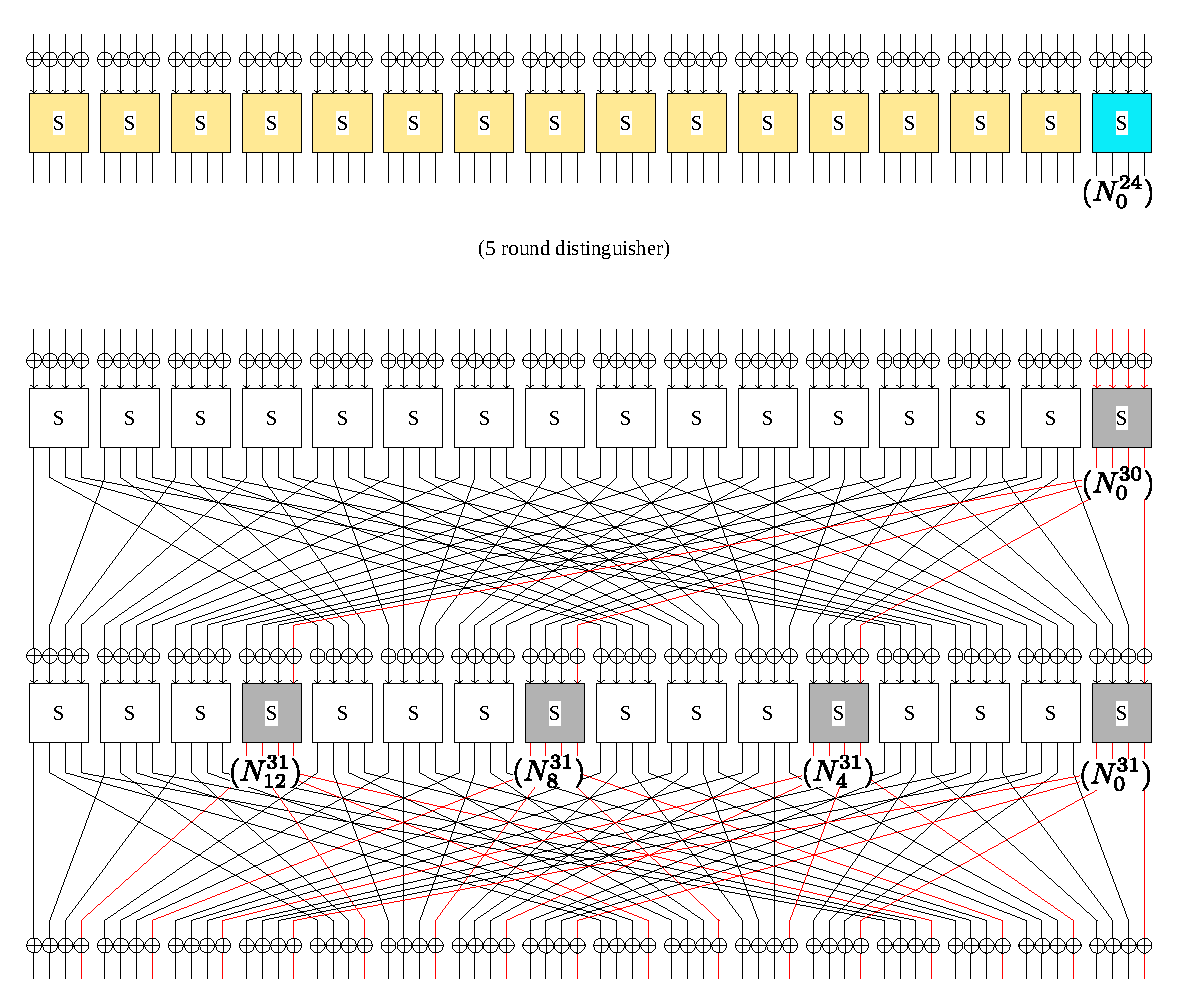
\includegraphics[width=\linewidth]{fig/spn_code_libra_2_round_attack.pdf}
	\caption{2 rounds key recovery attack on \present}
	\label{fig:key_recovery_2_round_present}
\end{figure}




\section{Balancedness in \gift cipher}	\label{sec:gift_random_nibble_explanation}
In this section we discuss about a to 5 round property of \present which is discussed in the section \autoref{sec:present_random_nibble_explanation}. Both \present and \gift uses SPN structure where the premutation layer is only bit permutation. Due to different bit permutation and \sbb of \present and \gift, for \gift 64 we get in total 16 balanced bits after 5 roundds. This is also a random nibble property i.e. it is irrespective of in which nibble we give All property at the input. We always get balanced bits at those particular 16 bits.

Initially we give the All property at the input of 0th nibble (as shown in fig \autoref{fig:gift_active_bit_propagation}). From the monomial representation of Division property we can say that, those bits will be unknown whose ANF representation contains $x_3x_2x_1x_0$. After 1st round the representation of bits of $N_0^0$ will be .......... After permutation layer, those 4 bits from $N_0^0$ goes to nibble 0, 4, 8, 12 \sbb contains constant combination of $y_3y_2y_1y_0$ in the ANF representaiton of their bits. So, the input of 3rd round contains combination of $y_3y_2y_1y_0$ as shown in \autoref{fig:gift_active_bit_propagation}. After the permutation of 3rd round we can see the 0th bits of the \sbb es goes to nibble 0, 1, 2, 3 in the next round (input of green color \sbb es in round 4). Similarly 1st, 2nd and 3rd bits of the \sbb es afer permutation layer of 3rd round goes to red, blue and yellow \sbb es respectively. The ANF of input bits of each green \sbb es in the 4th round is $(c_0 + c_1y_0, c_2 + c_3y_1, c_4 + c_5y_2, c_6 + c_7y_3)$ respectively. At the output of 4th round, each bit contains combination of $y_3y_2y_1y_0$ in their ANF representaion. As the input bits of the nibble for different colored \sbb es are same, their output also remains same without constants. Now in \gifts's \sbb ANF representation, lowest degree term appears for 0th and 1st bits. But if we consider 2 rounds the possibility of not containing the product term $x_3x_2x_1x_0$ is higher for 0th bit. This is because the 2 degree term of 0th bit contains 0th bit and 1st bit from the last round and both of them are 2-degree term too. Whereas the 1st bit contains previous round's 0th and 2nd bit term in 2-degree but 2nd bit contain s a 3rd degree term in the last round. For this, after two rounds the chances of getting balancedness at 0th bit is higher than other bits. We implemented this in Sage and compute the ANF's of the bits after 5 rounds. We see that after permutation layer of 5th round, the 0th bit of each \sbb does not contain the product term $x_3x_2x_1x_0$. The other bits ANF contains the term. Hence the 0th bits of each nibble becomes balanced after 5 rounds.



\begin{figure}[!h]
	\centering
	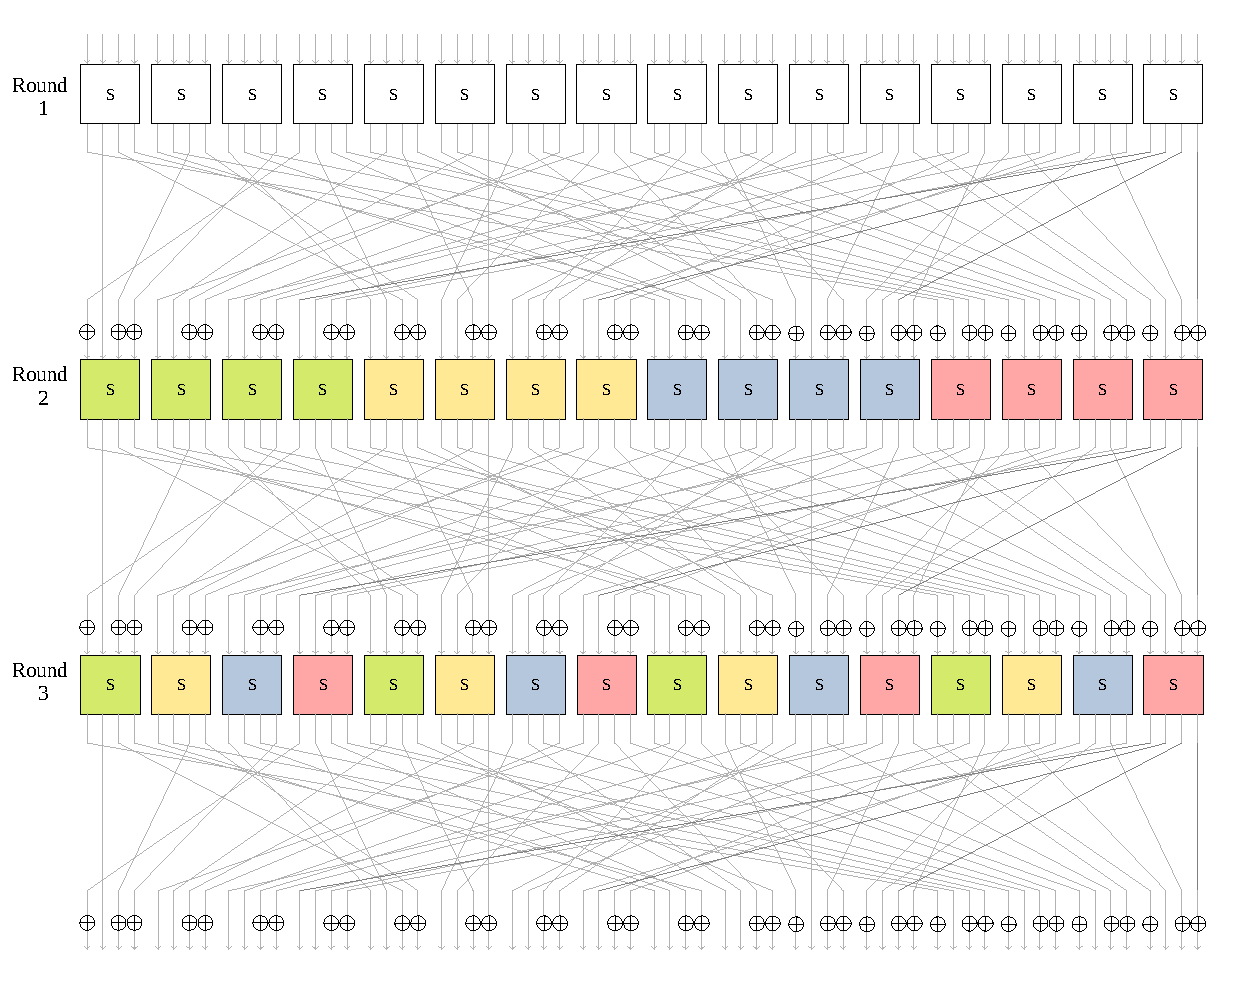
\includegraphics[width=\linewidth]{fig/gift_cipher_active_bit_propagation_random_nibble.pdf}
	\caption{random nibble active bit propagation on \gift}
	\label{fig:gift_active_bit_propagation_random_nibble}
\end{figure}




In the previoues paragraph we show the propagation after giving the All property at 0th nibble. Now we show that if we give All property at any random nibble then also, the same 16 bits becomes balanced. Suppose we give All at input of round 1 in nibble 0, 4, 8, 12. Then after permutation in the input of round 2, one of red nibble, blue yellow and green contains a constant combination of bit $y_0, y_1, y_2, y_3$ respectively. If we give All at nibble (1, 5, 9, 13) then input bit sequence at red, blue, yellow and green nibbles becomes ($y_0, y_1, y_2, y_3$), ($y_1, y_2, y_3, y_0$), ($y_2, y_3, y_0, y_1$), ($y_3, y_0, y_1, y_2$) respectively. So, we get a 4 bit sequence for giving All at any nibble in round 1. In the output of round 3 for each bit in nibble 0, 1, 2, 3 we get the ANF as constant combination of one of ($y_0, y_1, y_2, y_3$), ($y_1, y_2, y_3, y_0$), ($y_2, y_3, y_0, y_1$), ($y_3, y_0, y_1, y_2$). So in the input of round 4, for nibble 0, 1, 2, 3 we get one of the ANF of the anf sequence which is shown in \autoref{fig:gift_active_bit_propagation}. These 4 ANF sequences leads to the balancedness of 0th bit after 5th round. This is shown in the previous paragraph.



\begin{figure}[!h]
	\centering
	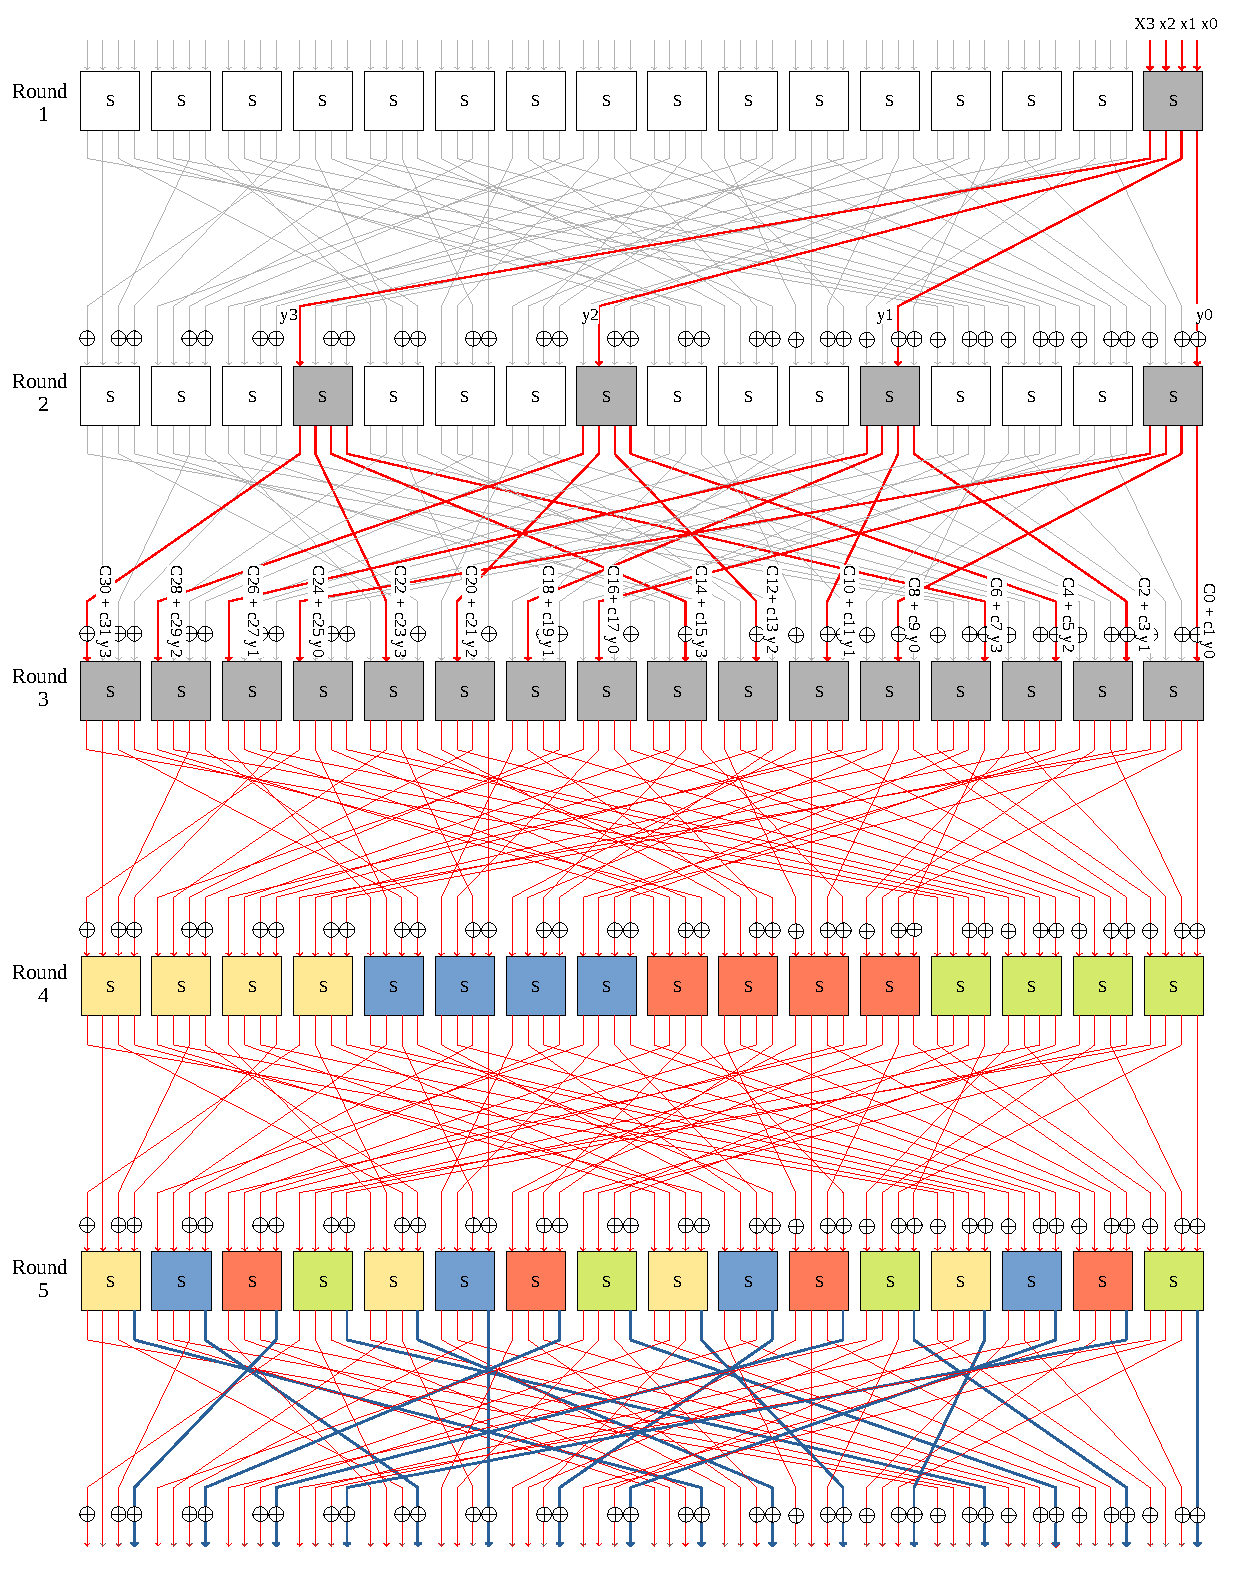
\includegraphics[width=\linewidth]{fig/gift_cipher_active_bit_propagation.pdf}
	\caption{active bit propagation on \gift}
	\label{fig:gift_active_bit_propagation}
\end{figure}





\begin{algorithm*}[htbp]
	\caption{\textsc{Key Recovery} ($C^\prime_1, \cdots, C^\prime_{16}$)}
	\label{alg:key_recovery_1_round_gift}
	\begin{algorithmic}[1]	
		\State Initialize an array called key\_list	
		\For{each key\_nibble in range\{$0$ - $4$\}}	\Comment{output of $SB$ at $N_0^{31}$ in fig.  \ref{fig:gift_key_recovery_1_round}}
			\For {each $j$ in range \{$0$ - $16$\}}
				\State dec\_msg[j] $\gets$ $SB^{-1}$(key\_nibble$\oplus$ $\text{perm}^{-1}(C^\prime_j$))
				\EndFor
			xor\_sum $\gets$ dec\_msg[0] $\oplus$ $\cdots$ $\oplus$ dec\_msg[15]
			\If{0th bit of xor\_sum is 0}	\Comment{input of $SB$ at $N_0^{31}$ in fig. \ref{fig:gift_key_recovery_1_round}}
			\State store \{key\_nibble\} in key\_list
			\EndIf
		\EndFor
		\Return key\_list			
	\end{algorithmic}
\end{algorithm*}






%\section{Balanced bits of smaller versions of present}
%
%\section{0th balanced bit of small present Present and gift ( to show the theory of monomial prediction )}

\section{DTM of each models}

